\section*{Einleitung und Hintergrund zur Wetterstation Arbon}
\addcontentsline{toc}{section}{Einleitung}

Die Wetterstation Arbon wurde 2005 als Lehrlingsarbeit des Berufsbildungszentrums Arbon auf Initiative der Technischen Gesellschaft Arbon (TGA) aufgebaut und in Betrieb genommen. Sie bestand aus mehreren Wettersensoren und einer Webcam, die auf einer Plattform auf dem See draussen montiert waren. Mit der Zeit haben sich immer mehr Probleme eingestellt. Grund waren einerseits nicht mehr funktionierende Sensoren, aber auch die selbstgeschriebene Software, die nicht mehr kompatibel war mit den neueren Betriebssystem-Versionen. Die Wetterstation wurde deshalb Ende 2013 ausser Betrieb genommen.

Ein Teil der Hardware und die komplette Software wurde 2015 von einer Gruppe Freiwilliger durch Standardhard- und Software ersetzt. Der Nachteil war aber, dass Messgrössen wie Pegel und Wassertemperatur nicht mehr gemessen werden konnten. Ausserdem basierte die of-the-shelf-Software auf Adobe Flash, was diverse Nachteile mit sich brachte. Eine detaillierte Analyse der Probleme findet sich in Fachmodul-Bericht\cite{BilWie2018MUIu}.

\vspace{5mm} %5mm vertical space
\begin{figure}[htbp!]
	\centering
	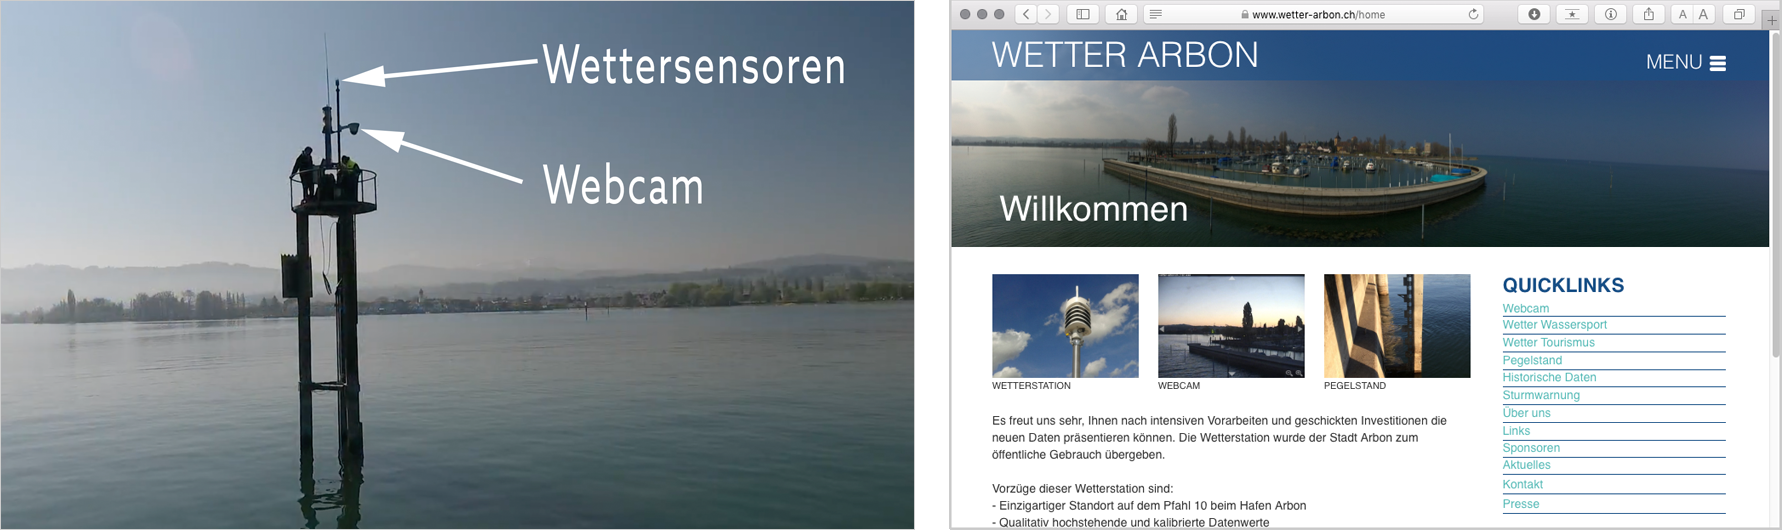
\includegraphics[width=1\linewidth]{img/kombi}
	\caption{Installation und Webseite der Wetterstation Arbon}
	\label{img:wetterstation}
\end{figure}
\vspace{3mm} %5mm vertical space

\noindent
Während der Bachelor-Arbeit wurde nicht nur Adobe Flash abgelöst sondern auch diverse Modernisierungen und Funktionserweiterungen hinzugefügt. Es wurden sowohl an der Hardware der Wetterstation, als auch an der Software Änderungen durchgeführt und dies auf der Webseite wie auch auf dem Server. Die verschiedenen Arbeiten wurden in sechs Blöcke unterteilt: Hardware, Webseite, Server, Programmierschnittstelle (API), Alarm-Meldungen (Benachrichtigungsservice) und Webcam. (vgl. Abb.\,\ref{img:module}). In den folgenden Kapiteln werden die einzelnen Blöcke genauer erläutert.

\vspace{5mm} %5mm vertical space
\begin{figure}[htbp!]
	\centering
	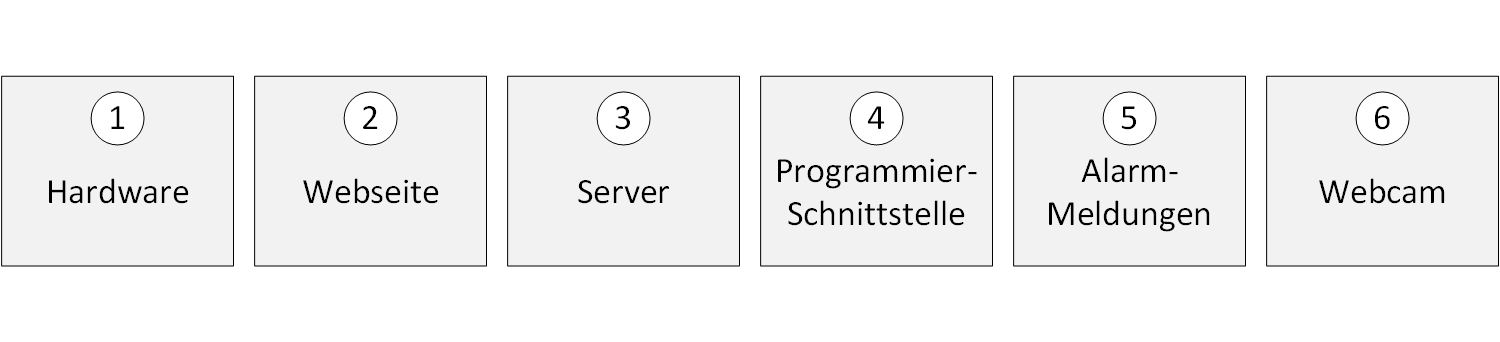
\includegraphics[width=1\linewidth]{img/module}
	\caption{Aufteilung der Arbeitsblöcke}
	\label{img:module}
\end{figure}
\newpage
